
\documentclass[12pt,a4]{article}
\usepackage{geometry}
 \geometry{
 a4paper,
 total={210mm,297mm},
 left=25mm,
 right=25mm,
 top=25mm,
 bottom=25mm,
 }
\usepackage{setspace}
\usepackage{graphicx}
\graphicspath{ {images/} }
\usepackage{epstopdf}
\DeclareGraphicsExtensions{.pdf,.eps}
\setlength\parindent{0pt}
\pdfimageresolution=300
\usepackage{lscape}
\usepackage{pdflscape}
\usepackage{amsmath} % Til generel matematik
\usepackage[utf8]{inputenc} % Til ÆæØøÅå
\usepackage{float}
\usepackage{standalone}
\usepackage{caption}
\captionsetup{labelfont = bf}
\newcommand\fnote[1]{\captionsetup{font=small}\caption*{#1}}
\setlength\parindent{24pt}
\linespread{1.3}
\usepackage[style=authoryear-comp,sorting=nty, backend=bibtex, maxcitenames=2]{biblatex}
\usepackage{pdfpages}

\addbibresource{C:/Users/ex-bce/Desktop/Revolving_Door/Determinants_of_Career_Choice/LaTeX/refs_for_career_choice.bib}

\begin{document}


\begin{figure}[H]
	\centering
	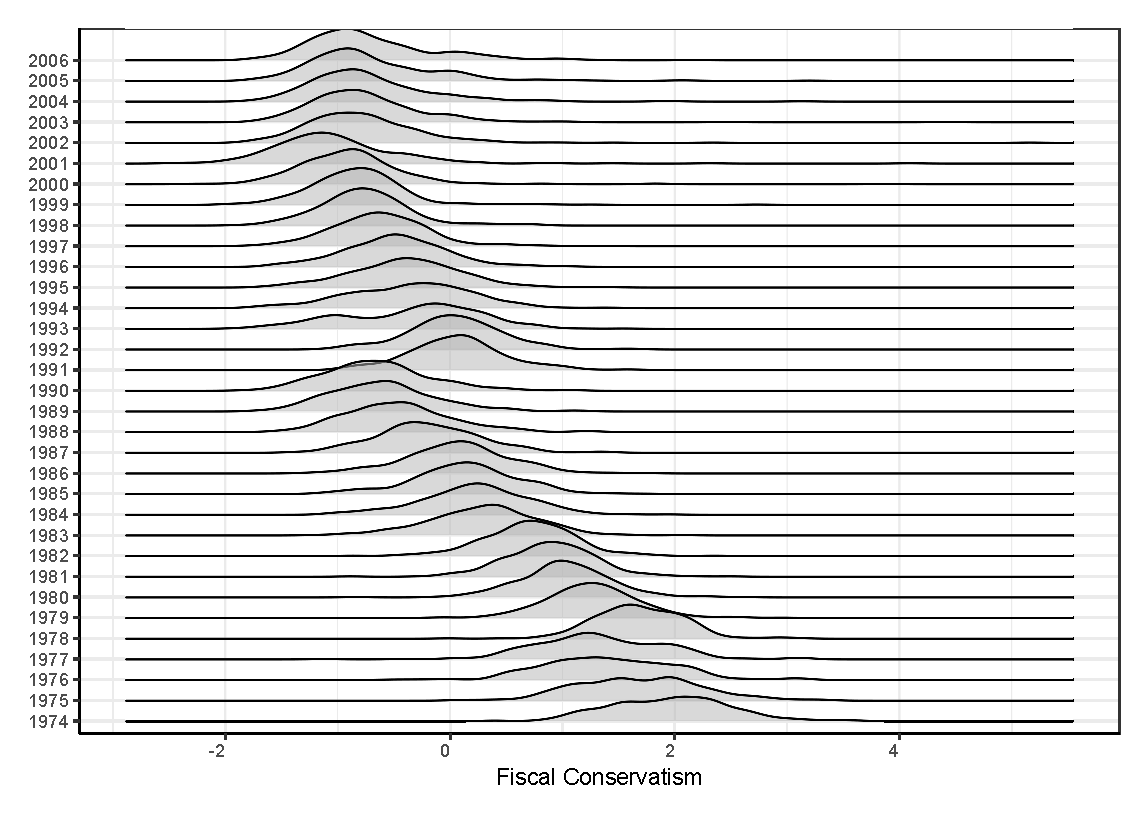
\includegraphics[scale = .8]{JoyPlotFiscal.eps}
	\caption{\textbf{.}} \fnote{ \emph{Note: .}}
	\label{fig:bar}
\end{figure}


\begin{figure}[H]
	%\centering
	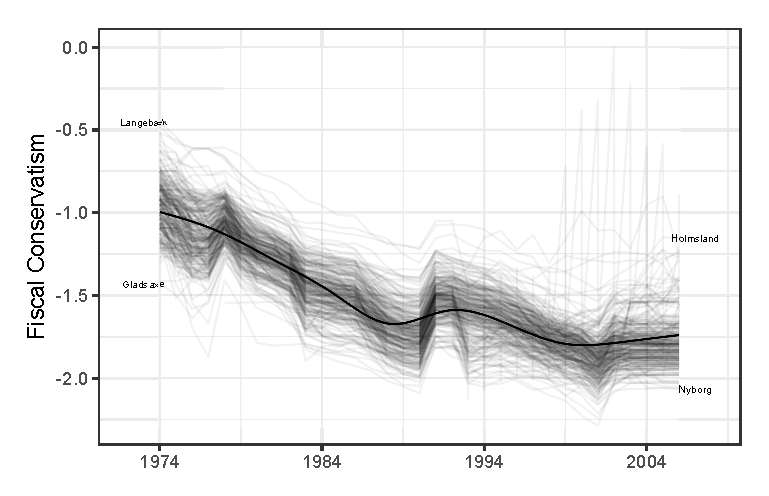
\includegraphics[scale = 1.2]{times_lines.eps}
	\caption{\textbf{Fiscal Conservatism in Danish Municipalities Across time.}} \fnote{ \emph{Note: .}}
	\label{fig:bar}
\end{figure}


\begin{landscape}
	\begin{figure}[H]
		%\centering
		\includegraphics[scale = 1.15]{Map_of_FiscCon.eps}
		\caption{\textbf{Mapping Fiscal Conservatism in Danish Municipalities: Three points in time.}} \fnote{ \emph{Note: .}}
		\label{fig:bar}
	\end{figure}
\end{landscape}	

\begin{figure}[H]
	%\centering
	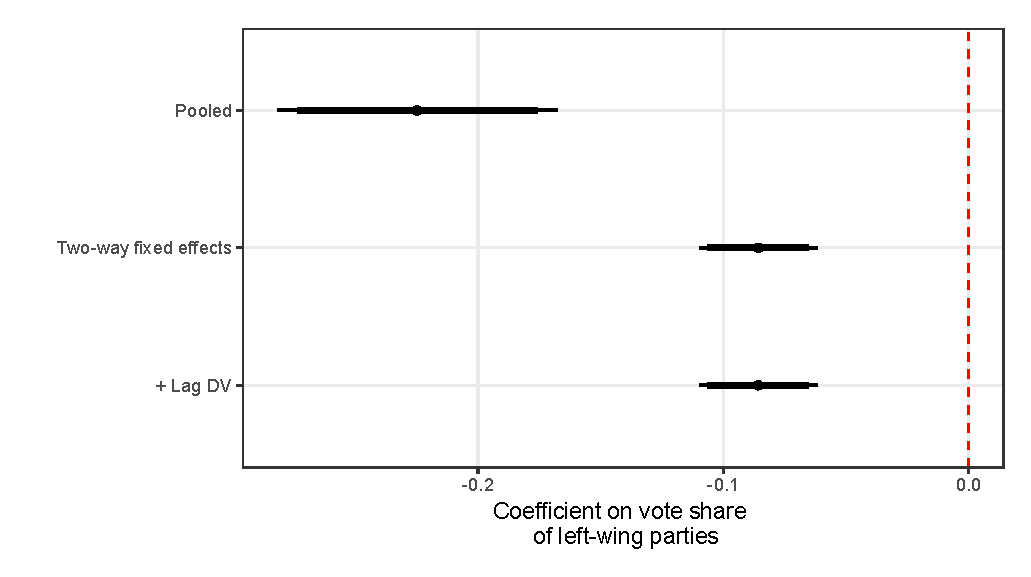
\includegraphics[scale = 1]{ggplot_coef.eps}
	\caption{\textbf{.}} \fnote{ \emph{Note: .}}
	\label{fig:bar}
\end{figure}	


\begin{figure}[H]
	%\centering
	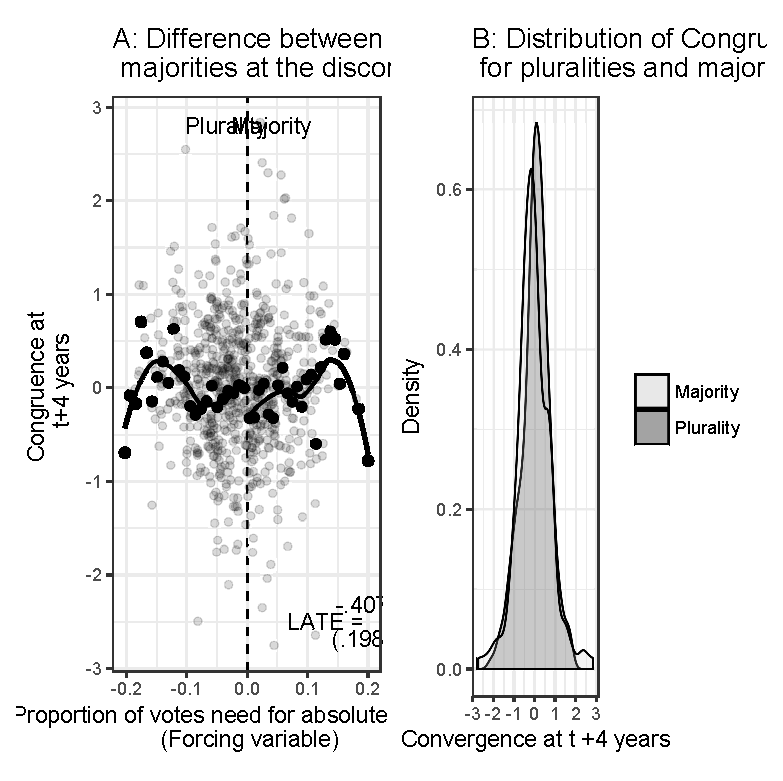
\includegraphics[scale = .75]{rddCongruence.eps}
	\caption{\textbf{.}} \fnote{ \emph{Note: .}}
	\label{fig:bar}
\end{figure}
	
	
\end{document}